\documentclass[11pt,a4paper]{article}
\usepackage[margin=24mm,headheight=15pt]{geometry}
\usepackage[T1]{fontenc}
\usepackage{mathpazo,helvet,courier}
\usepackage{graphicx,booktabs,longtable,array,amsmath,amssymb,xcolor,float,fancyhdr,titlesec,hyperref}
\definecolor{ink}{HTML}{243746}
\definecolor{accent}{HTML}{256B91}
\definecolor{rust}{HTML}{B35828}
\hypersetup{colorlinks=true,linkcolor=accent,urlcolor=accent,citecolor=accent,pdftitle={Rating shifts without identified skill shifts},pdfauthor={nakshatra0904}}
\titleformat{\section}{\Large\sffamily\bfseries\color{ink}}{\thesection}{.6em}{}
\titleformat{\subsection}{\large\sffamily\bfseries\color{ink}}{\thesubsection}{.6em}{}
\pagestyle{fancy}\fancyhf{}\fancyhead[L]{\small\sffamily Chess rating policy and measurement}\fancyhead[R]{\small\sffamily Empirical report}\fancyfoot[C]{\thepage}
\setlength{\parindent}{0pt}\setlength{\parskip}{6pt}
\renewcommand{\arraystretch}{1.15}
\setlength{\emergencystretch}{3em}
\newcommand{\note}[1]{{\small\color{ink} #1}}
\begin{document}
\hypersetup{pageanchor=false}
\begin{titlepage}
\vspace*{1.1cm}
{\sffamily\color{accent}\large ONLINE CHESS / APPLIED ECONOMETRICS\par}
\vspace{1cm}
{\sffamily\bfseries\color{ink}\fontsize{30}{36}\selectfont Rating shifts without identified skill shifts\par}
\vspace{.7cm}
{\sffamily\Large A difference-in-differences study of control-group sensitivity, participation, and post-game measurement around Chess.com's September 2020 reform\par}
\vspace{1cm}
{\large Research and analysis by nakshatra0904\par}
{\large R edition revised 12 October 2026\par}
\vfill
\rule{\textwidth}{.7pt}
\vspace{.3cm}
\textbf{Main research question}\par
How much does an apparent rating-policy effect depend on the comparison pool, the players included, and the timing of the rating measurement?\par
\vspace{.3cm}
\textbf{Data window}\par
1 June--31 October 2020. Public monthly Chess.com game archives, retrieved for a deterministically selected cohort.\par
\vspace{.3cm}
\textbf{Evidence standard}\par
I estimate a difference-in-differences model, examine an event study and placebo breaks, and audit rating measurement. I distinguish empirical findings from the assumptions required for causal interpretation.\par
\end{titlepage}
\pagenumbering{roman}\hypersetup{pageanchor=true}
\begingroup\small\setlength{\parskip}{0pt}\tableofcontents\endgroup\clearpage\pagenumbering{arabic}

\section{Executive findings}

I analyze 61,479 unique rated standard-chess games and 62,181 focal player-game observations from 120 July-active accounts, selected by screening 256 accounts from a 1,743-account grandmaster sampling frame. I investigate an administrative rating change and distinguish displayed rating increases from improvement in chess skill.

My primary two-way fixed-effects difference-in-differences (DiD) regression estimates a bullet-versus-blitz shift of \textbf{191.6 rating points}, with an exploratory player-clustered 95\% interval of [99.6, 283.6]. The estimation sample has 20 players and 485 observed player-pool-week cells. This conditional contrast is a cohort-specific estimate; the policy was one platform-wide event, so its uncertainty is not fully captured by treating players as independent policy replications.

A simpler matched-player calculation gives 183.6 points, with a player-resampling percentile interval of [132.1, 245.1]. The difference from the fixed-effects estimate reflects aggregation and weighting. Both estimates should be compared with the announced 150-point administrative offset, not interpreted as a gain of the same amount in latent ability.

The joint test of the five nearest pre-event contrasts has p = 0.602. This diagnostic does not establish parallel trends: pre-tests may have limited power, and multiple co-occurring reforms threaten the comparison even when a pre-test does not reject. I therefore estimate several control definitions, common-player comparisons, pre-period placebos, and a differential-trend sensitivity model.

The endpoint's ratings are recorded after the game. In 21,674 observed adjacent decisive rematches, I compare retrospective performance metrics using post-game and prior-rematch ratings. The equal-pair mean improvement in log loss is 0.0443, with a pair-resampling interval of [0.0436, 0.0450]. This is a measurement audit of information timing, not a new discovery that leakage can occur and not a deployable forecasting validation.

\textbf{The most useful distinction in this cohort.} Removing the directly reclassified 10|0 observations changes the main estimate by only 0.02 points. On the common 18-account sample, changing the comparator from all blitz to 3|0 changes it by about 1.1 points. In contrast, weighting cells by their number of games raises the estimate from 191.6 to 261.1 points. Thus weighting and participant support are more consequential than the direct 10|0 exclusion in this GM-oriented cohort; the result does not establish that comparator contamination is unimportant for the whole platform.

\textbf{Contribution.} Prior work already analyzes rating prediction and post-game leakage. My narrower contribution is a reproducible sensitivity study connecting an actual reform to comparator contamination, changing participation, and measurement timing. In a targeted search, I found no directly matching study of this exact combined design; that is a limited search finding, not proof of worldwide novelty.

\section{Earlier work and the refined research question}

\subsection{What has already been done?}

Rating models and their uncertainty are established subjects. Glickman's original Glicko formulation adds rating uncertainty to skill estimation \cite{glicko}. Current platform documentation distinguishes implementation details and player pools \cite{chessratings,lichessratings}. I use established rating theory and interpret Chess.com points within their own platform and rating pool.

Public applied projects also cover several obvious questions. Sharma's 2023 Chess.com analysis regresses rapid ratings on other ratings \cite{sharma}. The ChessIQ repository explicitly identifies outcome leakage from post-game ratings and PGN fields \cite{chessiq}. Smerdon's Fighting Chess Index demonstrates descriptive construction and regression adjustment of chess performance characteristics \cite{smerdon}. These are direct examples of earlier work; the latter two are public project or author publications, not evidence that every nearby question has been peer reviewed.

\begin{table}[H]\centering\small\caption{Related work and the narrower empirical contribution}\begin{tabular}{p{3cm}p{4.1cm}p{6cm}}\toprule

Earlier work & Relevant overlap & Distinction in this report \\ \midrule

Glickman, Glicko & Uncertainty-aware ratings & Empirical policy measurement \\

Sharma (2023) & Cross-pool regression & Historical within-player contrasts \\

ChessIQ project & Post-game rating leakage & Observed rematch audit near reform \\

Smerdon (2021) & Draw statistics and adjustment & Policy comparator sensitivity \\

DiD methods literature & Trends and dependent errors & Applied audit of one platform event \\

\bottomrule\end{tabular}\end{table}

\subsection{Search scope and what novelty can mean}

I searched the public web and consulted primary pages on 11 October 2026. Query families included Chess.com / September 2020 / rating / regression; bullet / 150 / difference-in-differences; chess / post-game rating / leakage; chess / rating inflation / empirical study; and Chess.com / September 10 / control group. I found direct prior work on two candidate topics and narrowed my initial generic rating-prediction question. The repository contains the query ledger and verified source links.

My search was targeted, not a systematic review of subscription databases, non-English theses, or every GitHub repository. I found no directly matched study in the results I reviewed. The appropriate novelty claim is therefore an original analysis of this frozen dataset and specification set, conditional on a documented search, rather than a claim that nobody has considered comparison-group sensitivity in chess.

\subsection{Main question and secondary questions}

The central question is whether the apparent effect of a common rating rebase remains similar when the comparison pool and participant mix change. The simultaneous reclassification of 10-minute chess makes blitz a potentially affected comparator. Restricting observations to unchanged time controls may reduce direct composition changes, while leaving pool-wide spillovers unresolved.

Three secondary questions are answered: (i) how much do game-weighted and equal-player comparisons differ; (ii) are first observed policy-crossing bullet changes compatible with an offset plus ordinary game updates; and (iii) how do result-associated rating updates alter performance metrics when measured ratings are used retrospectively? I defined all specifications before inspecting their estimated policy coefficients. I expanded the cohort from 128 to 256 screened accounts after observing activity counts, to improve coverage, without using estimated effects as a stopping rule.

\section{Policy context and what a rating measures}

Chess.com's 10 September 2020 announcement describes two changes: 10|0 games moved from blitz to rapid, and active bullet ratings received an administrative increase of 150 points. The bullet adjustment was applied on a subsequent live-chess login, with a short rollout delay. Eligible rapid ratings could also be raised to the player's higher blitz rating \cite{policy}. The announcement date is therefore an intention-to-treat time marker, not an observed account-level treatment timestamp.

A rating is an estimated coordinate within a population and implementation. A uniform offset $c$ applied to both players leaves their difference unchanged: $(r_i+c)-(r_j+c)=r_i-r_j$. Any expectation formula depending only on the difference is invariant to this common rebase. An increase in displayed points can thus be mechanically large while implying no change in relative expected score.

For illustration, the Elo-shaped curve is $E_i=1/(1+10^{-(r_i-r_j)/400})$. A hypothetical update $r_i'=r_i+K(s_i-E_i)$ would depend on both result and expectation. This is an illustrative formula, not a reconstruction of Chess.com's Glicko updates. Historical rating deviation, update parameters, refunds, and exact login time are absent from the archives used here.

\begin{figure}[H]\centering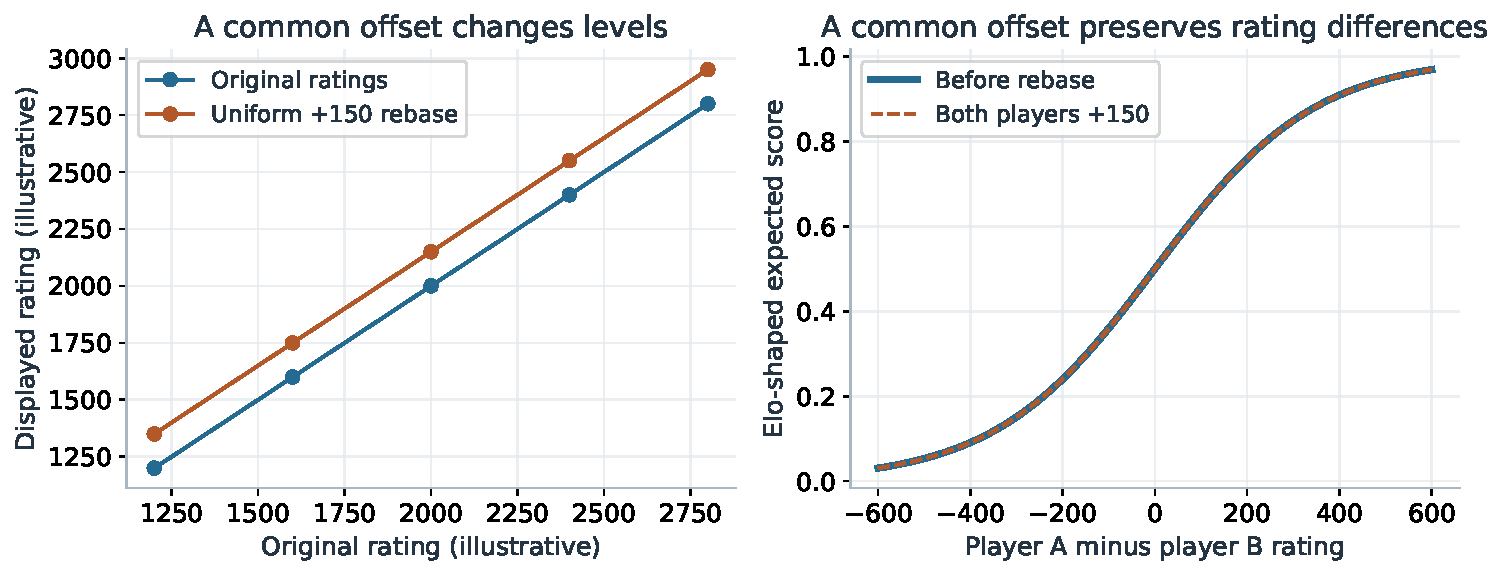
\includegraphics[width=\textwidth]{figures/12_rebase_invariance.pdf}\caption{Illustrative mechanism, not empirical observations: a uniform 150-point offset changes absolute levels but preserves pairwise differences. The curve is Elo-shaped and is not fitted to the cohort.}\end{figure}

Two timing details matter. First, the documented monthly-game JSON ratings are post-game measurements. Second, the PGN rating headers in these data match those JSON values. Treating them as pre-game inputs would import information generated by the outcome into an apparent prediction exercise \cite{pubapi}. I use them as measured outcomes in the policy analysis and interpret the logistic regression as retrospective association.

\section{Data collection, provenance and sample construction}

\subsection{Reproducible sampling}

The public GM-title endpoint contained 1,743 account names at retrieval. I ranked each normalized name by the SHA-256 digest of the fixed string \texttt{chess-policy-2020-v1|} followed by that name. The first 256 names formed the screening sample. Accounts with at least one rated standard bullet, blitz, or rapid game in July 2020 formed the historical active cohort (120 accounts). I retrieved complete available archives for June, July, August, September, and October 2020 for those accounts.

This is deterministic pseudo-random selection from a contemporary title list, followed by historical activity screening. It is not a probability sample of all 2020 Chess.com users. Accounts that no longer appear in the current frame can be missing; players may have earned titles later; and inactive July accounts are deliberately excluded. Public handles identify accounts, not necessarily distinct people. I do not assume that these accounts already held GM titles in 2020.

\subsection{Cleaning and observational units}

I retain rated standard chess in the three live speed classes, interpret White's result as 1, 0.5, or 0, require numeric ratings between 100 and 4000, normalize usernames, and deduplicate by game UUID (falling back to URL). I exclude variant chess, daily chess, unrated games, and unknown final results. I convert game finish timestamps to UTC; the window ends before 1 November 2020.

I maintain two distinct observational units. The unique-game file contains each game once, even when both players are sampled. The focal player-game file contains one row for each sampled participant. A game with two cohort accounts contributes two focal rows but only one unique-game row. Descriptive participant ratings use the latter focal unit; win/draw summaries and outcome regressions use unique games. This prevents duplicate games from being treated as independent outcome observations.

\begin{table}[H]\centering\small\caption{Sample construction and audit counts}\begin{tabular}{lr}\toprule

Stage / property & Count \\ \midrule

Current GM account frame & 1,743 \\

Accounts screened & 256 \\

July-active cohort accounts & 120 \\

Retrieved archive game records & 68,920 \\

Rejected archive rows & 6,718 \\

Repeated eligible archive appearances removed & 723 \\

Unique eligible games & 61,479 \\

Focal player-game observations & 62,181 \\

Primary panel players & 20 \\

Primary panel cells & 485 \\

\bottomrule\end{tabular}\end{table}

The observed eligible timestamps run from 2020-06-01 07:02:08+00:00 to 2020-10-31 23:35:57+00:00. PGN and JSON rating values match in 100.00\% of unique games. Request URLs, retrieval times, status codes, content hashes, the frozen sampling frame, and the selected cohort are included. I record unavailable archives as missing and do not impute their games.

\subsection{Descriptive statistics}

\begin{table}[H]\centering\small\caption{Published post-game ratings among focal observations, June--October 2020}\begin{tabular}{lrrrrrrr}\toprule

Pool & Obs. & Accounts & Mean & Median & SD & P10 & P90 \\ \midrule

blitz & 41,263 & 115 & 2,651.6 & 2,663.0 & 161.1 & 2,434.0 & 2,851.8 \\

bullet & 20,189 & 73 & 2,570.0 & 2,572.0 & 143.6 & 2,406.0 & 2,737.0 \\

rapid & 729 & 61 & 2,364.5 & 2,373.0 & 238.8 & 2,071.8 & 2,673.0 \\

\bottomrule\end{tabular}\end{table}

These are game-weighted statistics: a frequent player contributes more observations. The distribution describes this selected cohort's activity, not platform-wide percentiles. Standard deviation describes observed dispersion and is not a standard error. Game outcomes, repeated opponents, and account activity induce dependence that is addressed in model uncertainty only to the extent described below.

\begin{figure}[H]\centering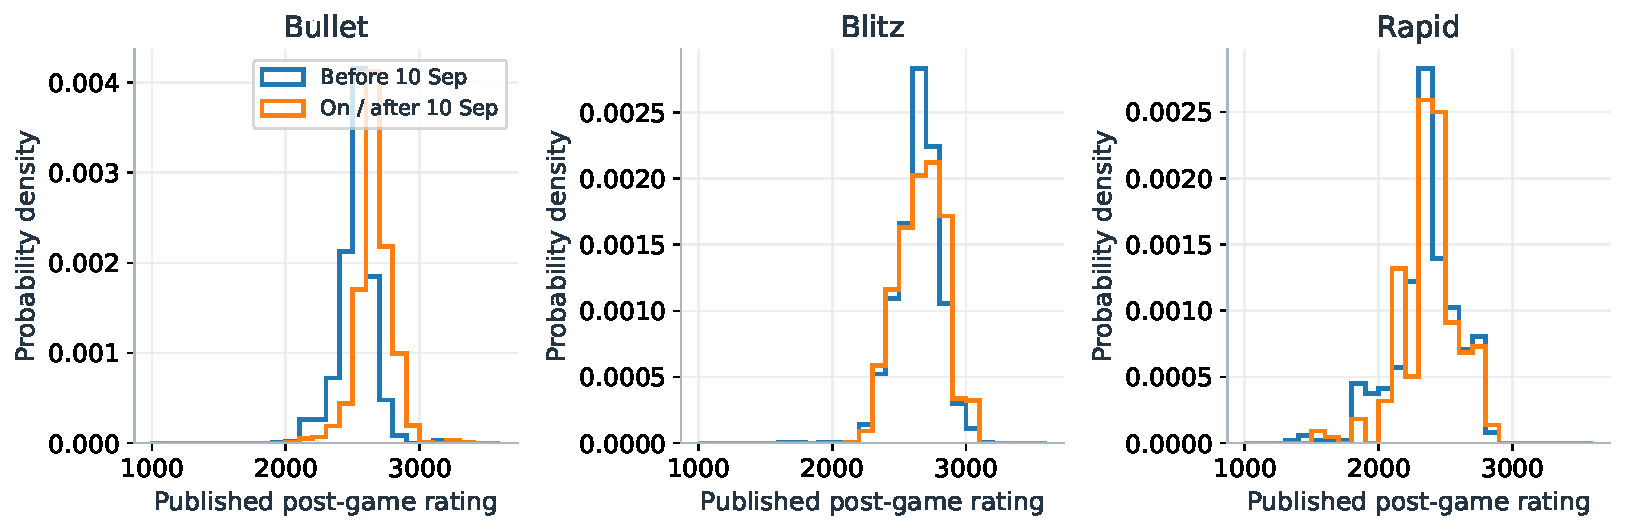
\includegraphics[width=\textwidth]{figures/02_distributions.pdf}\caption{Focal post-game rating distributions before and on/after 10 September 2020. Frequency polygons use 100-point bins and are normalized within pool-period. Source: frozen Chess.com cohort archives, June--October 2020.}\end{figure}

\section{Difference-in-differences design and assumptions}

\subsection{Two-way fixed-effects DiD specification}

I anchor seven-day event bins at 00:00 UTC on 10 September 2020. Week $k=\lfloor(t-t_0)/7\text{ days}\rfloor$ is based on game completion time. I omit week 0 (10--16 September) from panel estimation because treatment timing is imprecise. My main panel retains player-pool-week cells containing at least three focal games. Each retained account must have observed qualifying bullet and blitz cells in both periods; it need not appear in every week.

I use difference-in-differences: bullet is the treated pool and blitz is the comparison pool for the same accounts. I compare their changes before and after the announcement, excluding the rollout week. My two-way fixed-effects least-squares specification is
\begin{equation}
\bar R_{ict}=\alpha_{ic}+\lambda_t+\beta\,\mathbf{1}(c=\mathrm{bullet})\mathbf{1}(t\geq1)+\varepsilon_{ict}.
\end{equation}
Here $\alpha_{ic}$ is a player-by-pool fixed effect, $\lambda_t$ is an event-week fixed effect, and $\bar R$ is the mean published post-game rating in the cell. Observed cells receive equal weight. I also estimate a sensitivity model weighted by game count; neither weighting guarantees representativeness.

The coefficient compares the change in bullet with the contemporaneous change in blitz after accounting for persistent player-pool levels and common weekly shifts. Its causal interpretation would require parallel untreated trends in bullet versus the chosen control, no relevant spillovers into blitz, no differential measurement changes, and ignorable changes in observation. These requirements are not secured by the public data.

\subsection{Uncertainty and diagnostic tests}

I calculate regression intervals with the R cluster-robust sandwich covariance, clustering by account and using a Student-$t$ reference with the cluster degrees-of-freedom correction \cite{rstats,zeileis}. I additionally bootstrap entire player contrasts 10,000 times using seed 20201011 and R's Mersenne-Twister generator. The resampling intervals are recomputed in R; identical integer seeds need not produce identical draws across software implementations. This retains within-player dependence, but is a different aggregate estimand from the fixed-effects coefficient. Bootstrap intervals use percentiles, not a claim of exact small-sample coverage.

Many games do not imply many independent policy changes. Players share opponents, pool dynamics, and a single announcement. Account clustering does not capture every cross-player shock. The econometric literature documents sensitivity to serial correlation and to having few policy changes \cite{bertrand,conley}. Reported intervals are useful cohort-level diagnostics and do not establish the uncertainty of a counterfactual platform-wide reform effect.

I estimate an event study interacting bullet status with each observed event week, relative to week -1. I jointly test the five contrasts for weeks -6 through -2 as a near-event pre-trend diagnostic. I use four earlier dates as placebo breaks, restricting their estimation to pre-announcement observations. Non-rejection is not proof of the identifying assumption, and post-selection on a pre-test can distort inference \cite{roth}. All these checks are exploratory, with no multiplicity-adjusted family-wise significance claim.

\subsection{Why a sharp regression discontinuity is not used}

There is no observed assignment score with a treatment threshold. Calendar time is shared by everyone and coincides with other platform changes, so a sharp regression discontinuity in time would require strong assumptions about contemporaneous shocks. I also do not infer treatment receipt from an outcome-derived rating jump: doing so would select treatment on the dependent variable. The date-indexed design is an announcement-based panel contrast.

\begin{figure}[H]\centering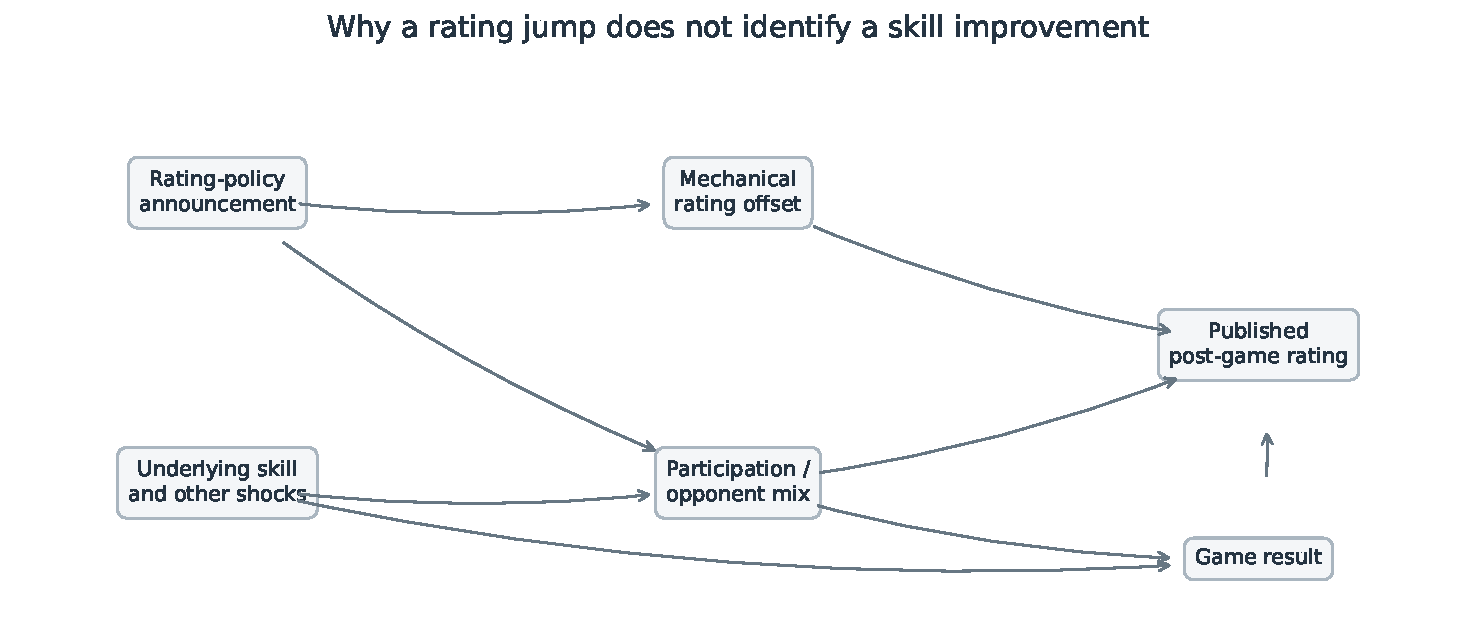
\includegraphics[width=\textwidth]{figures/13_causal_structure.pdf}\caption{Conceptual causal structure. Participation and opponent mix can affect measured ratings; game results also enter post-game ratings. The diagram summarizes mechanisms and is not an estimated causal graph.}\end{figure}

\section{Descriptive behavior around the announcement}

\begin{figure}[H]\centering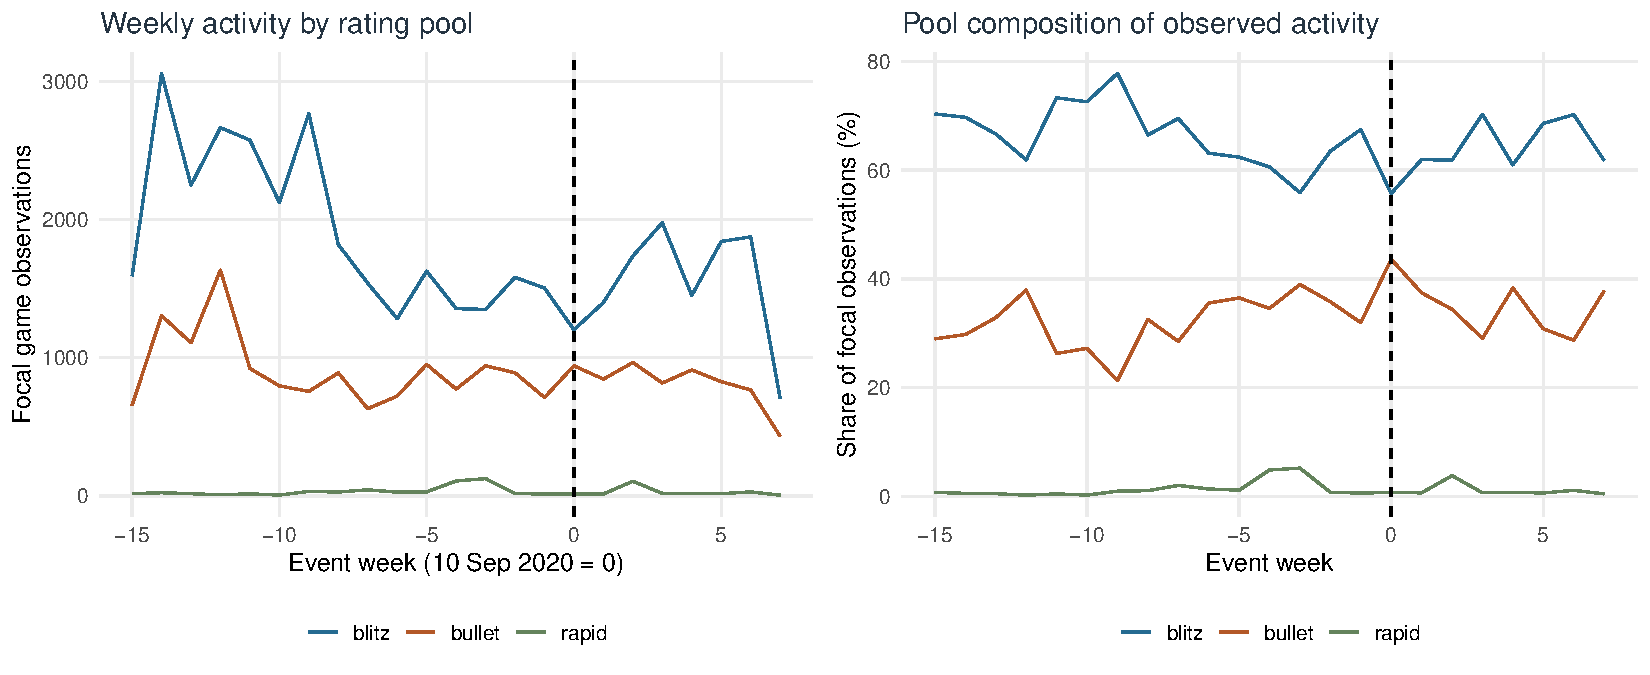
\includegraphics[width=\textwidth]{figures/01_activity.pdf}\caption{Focal game observations and their pool shares in anchored seven-day event bins. Boundary bins are incomplete calendar exposure; every series describes the sampled archives, not total site activity. Source: Chess.com archives, June--October 2020.}\end{figure}

The activity plot identifies changes in the observed mix before interpreting mean ratings. A higher mean can arise because stronger or more active accounts play more games, because players move between speed classes, or because the same players receive a rebase. Weekly game counts are descriptive; no exposure-adjusted behavioral treatment effect is estimated from these counts.

\begin{figure}[H]\centering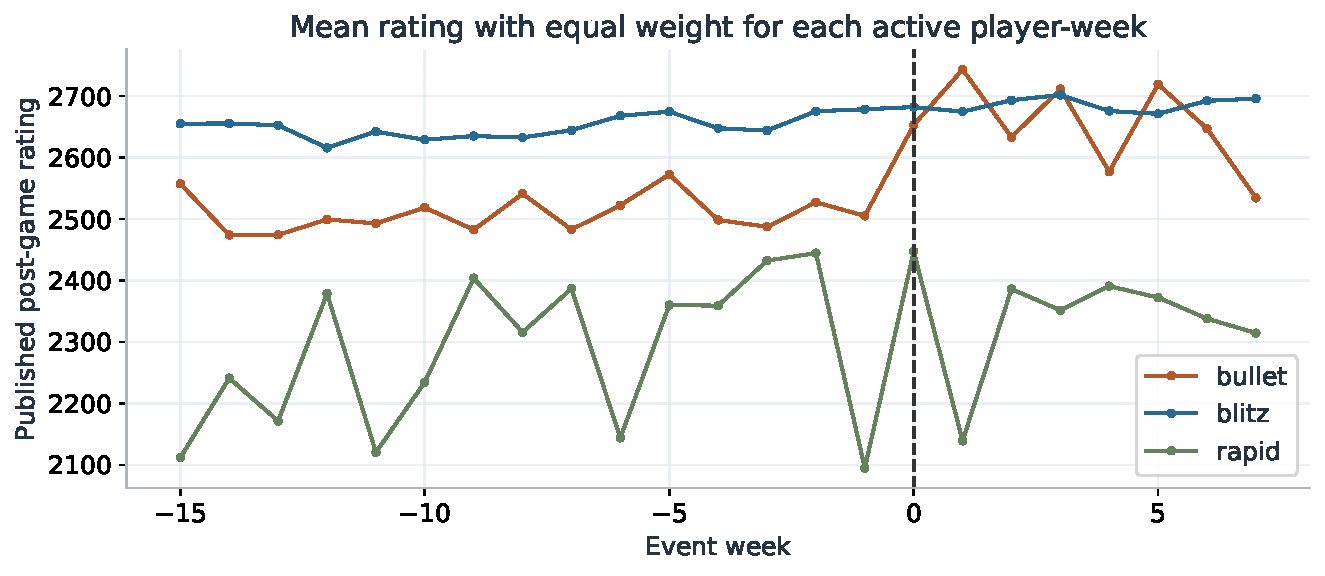
\includegraphics[width=\textwidth]{figures/03_rating_trends.pdf}\caption{Equal-account weekly means: each account with observed games in a pool-week contributes its own mean rating once. The set of accounts can change by week. Source: Chess.com cohort archives, June--October 2020.}\end{figure}

Equal-player weighting reduces domination by high-volume players but does not hold membership fixed. The fixed-effects panel and paired-player contrasts below address a different question: how observed ratings changed within accounts that appear in both periods and both main pools. A visual discontinuity in an unbalanced mean is therefore supporting description, not the identifying evidence.

\section{DiD estimates, event study and sensitivity}

My primary DiD estimate is 191.6 points (clustered SE 44.0; 20 account clusters). The estimate differs from the announced offset by 41.6 points. This discrepancy can reflect later ordinary rating updates, incomplete treatment exposure, the behavior of the comparison pool, and the sample weighting. It does not by itself demonstrate that Chess.com implemented the policy incorrectly.

\begin{table}[H]\centering\small\caption{Difference-in-differences estimates, in rating points; account-clustered intervals}\begin{tabular}{p{6.2cm}rrrr}\toprule

Specification & Estimate & 95\% interval & Players & Cells \\ \midrule

All blitz; balanced; >=3 games & 191.6 & 99.6 to 283.6 & 20 & 485 \\

Exclude 10|0; balanced; >=3 games & 191.6 & 99.6 to 283.6 & 20 & 485 \\

3|0 only; balanced; >=3 games & 196.2 & 95.6 to 296.7 & 18 & 421 \\

All blitz; unbalanced; >=3 games & 165.7 & 102.3 to 229.2 & 115 & 1,547 \\

All blitz; balanced; >=1 game & 163.7 & 102.9 to 224.4 & 31 & 780 \\

All blitz; balanced; +/-6 weeks & 204.0 & 104.7 to 303.3 & 13 & 197 \\

All blitz; differential linear trend & 185.1 & 117.3 to 253.0 & 20 & 485 \\

All blitz; game-count weighted & 261.1 & 113.2 to 409.0 & 20 & 485 \\

Common players: all blitz & 197.2 & 99.7 to 294.8 & 18 & 449 \\

Common players: 3|0 only & 196.2 & 95.6 to 296.7 & 18 & 421 \\

\bottomrule\end{tabular}\end{table}

\begin{figure}[H]\centering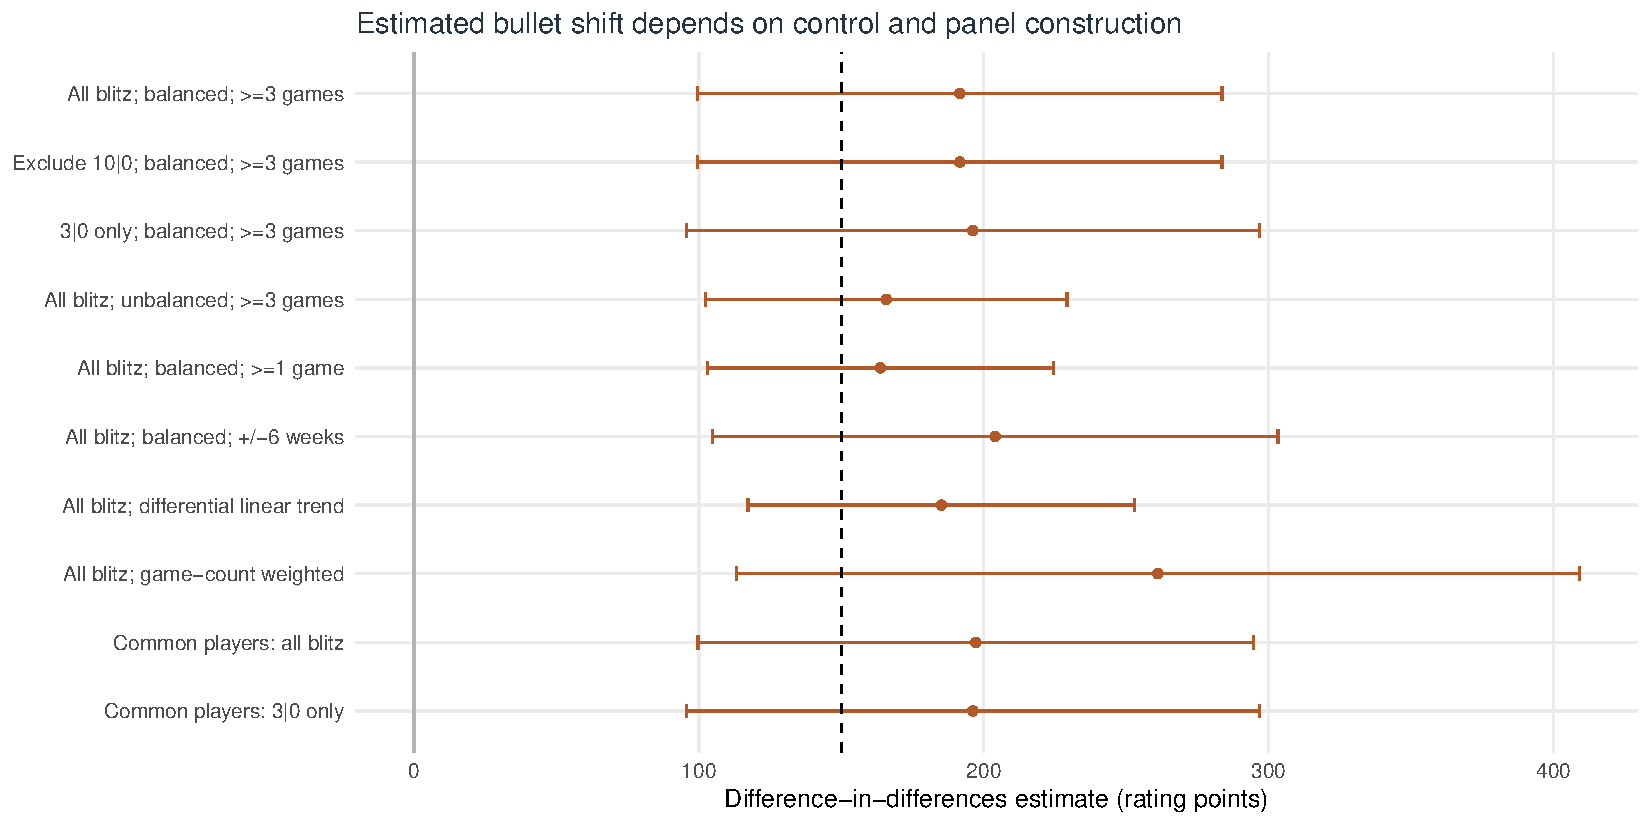
\includegraphics[width=\textwidth]{figures/04_did_sensitivity.pdf}\caption{Each marker is a separate player-pool-week fixed-effects estimate with an exploratory 95\% account-clustered interval. Some specifications change the eligible accounts as well as the controls. Source: Chess.com cohort archives, June--October 2020.}\end{figure}

The unchanged-control comparison restricts blitz to 3|0, while another specification excludes 10|0 only. My planned 5|0 comparison did not retain the minimum three eligible account clusters, so I omit that specification. These are controls defined by recorded game settings, not randomized comparison groups. The common-player pair of specifications holds the account set fixed between all-blitz and 3|0 comparisons, helping separate account selection from the choice of control observations. Weekly activity support may still differ.

The unbalanced model admits more player-pool trajectories; the one-game threshold retains noisier cells; the shorter window reduces long-run drift; the game-count weighting changes the target toward frequent play; and the differential linear-trend model allows bullet to drift differently before and after the break. These are substantive sensitivity checks, not independent confirmations. A trend model also imposes a functional form and can extrapolate a noisy pre-trend.

\begin{figure}[H]\centering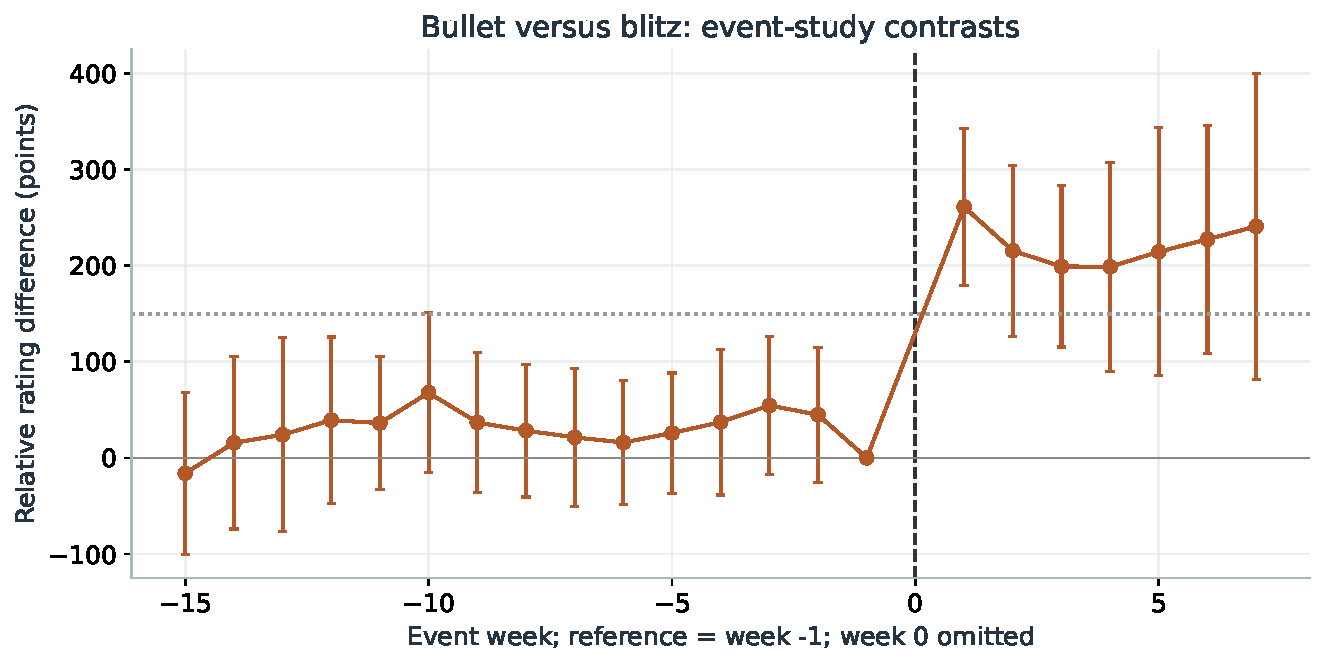
\includegraphics[width=\textwidth]{figures/05_event_study.pdf}\caption{Event-study bullet-versus-blitz contrasts relative to week -1. Week 0 is excluded. Bars are exploratory account-clustered 95\% intervals; the dotted 150-point line is a policy benchmark. Source: the primary cohort panel, June--October 2020.}\end{figure}

For the near-event pre-period joint test, p = 0.602. The full event-study path, including uncertainty, is more informative than treating that single number as a pass/fail gate. Persistent lead differences, wide intervals, or large placebo estimates weaken the case that an observed post-event change is attributable entirely to the announcement.

\begin{table}[H]\centering\small\caption{Pre-announcement placebo breaks, using the primary accounts and pre-period cells only}\begin{tabular}{rrrr}\toprule

Placebo event week & Estimate & 95\% interval & p-value \\ \midrule

-10 & 17.5 & -37.2 to 72.1 & 0.512 \\

-8 & -2.3 & -49.9 to 45.2 & 0.919 \\

-6 & 2.0 & -43.5 to 47.5 & 0.928 \\

-4 & 19.6 & -22.6 to 61.9 & 0.343 \\

\bottomrule\end{tabular}\end{table}

\begin{figure}[H]\centering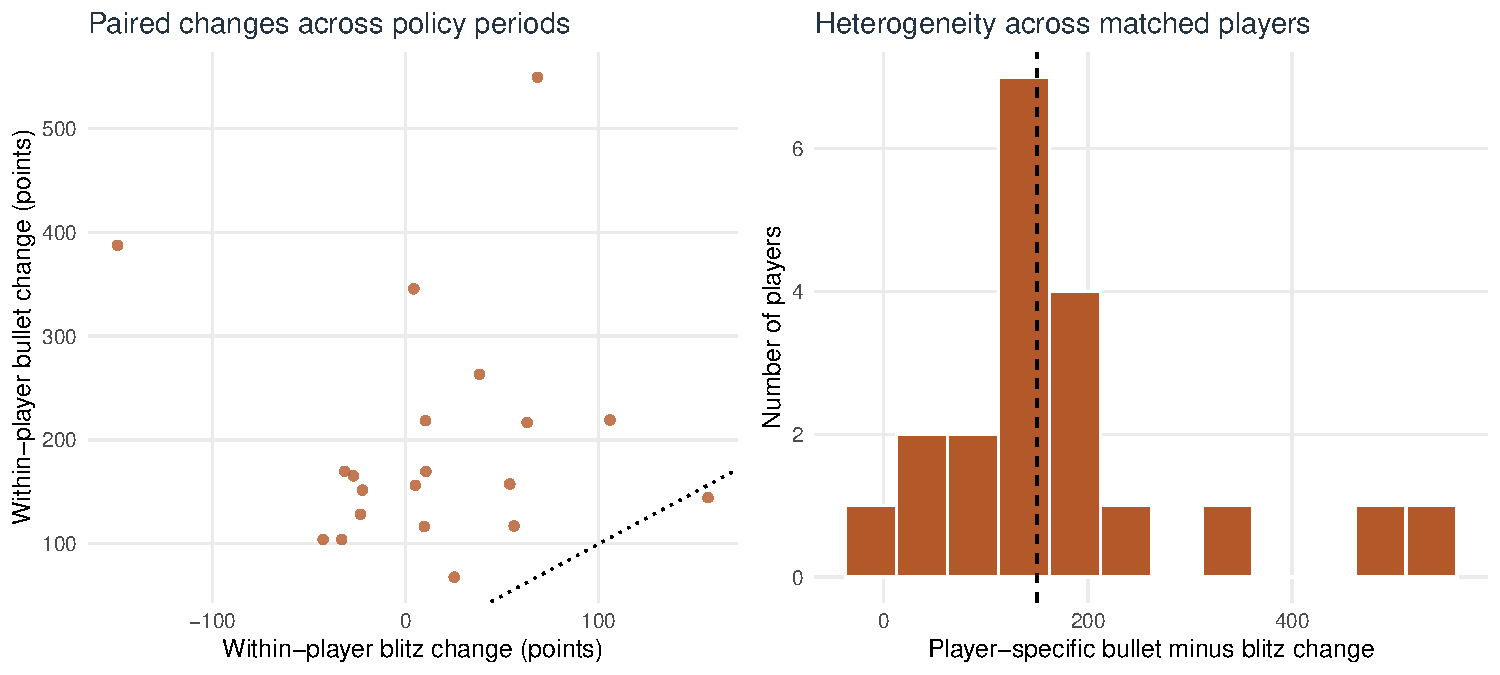
\includegraphics[width=\textwidth]{figures/06_player_changes.pdf}\caption{Each point is a matched account: equal-week post-minus-pre bullet and blitz changes. The right panel shows their differences; the 150-point line is an announced-offset benchmark. Source: the primary panel.}\end{figure}

The matched-player bootstrap estimate is 183.6 points, with interval [132.1, 245.1]. The player distribution makes heterogeneity visible. Accounts with large changes should not be labeled as unusually improved or as suspicious: the measure includes estimation noise, elapsed time, ordinary results, and selection into play.

\section{Participation, reclassification and the comparator problem}

\begin{figure}[H]\centering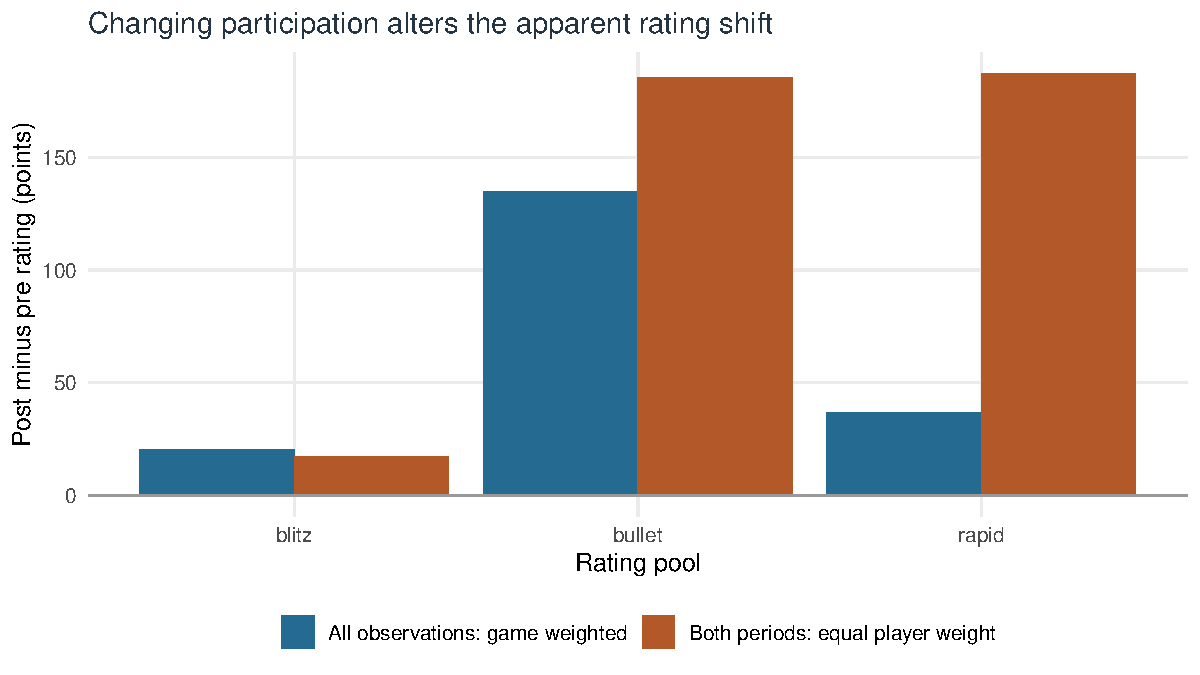
\includegraphics[width=\textwidth]{figures/07_composition.pdf}\caption{Two different descriptive estimands: all-game mean changes versus mean within-account changes among accounts observed in both periods. Their difference combines activity weighting and account composition. Source: Chess.com archives, June--October 2020.}\end{figure}

\begin{table}[H]\centering\small\caption{Participation and weighting contrasts; ratings in points, account counts at right}\begin{tabular}{lrrrrr}\toprule

Pool & All-game change & Matched change & Matched & Pre & Post \\ \midrule

bullet & 134.9 & 185.5 & 39 & 66 & 46 \\

blitz & 20.3 & 17.4 & 90 & 115 & 90 \\

rapid & 36.9 & 187.4 & 14 & 52 & 23 \\

\bottomrule\end{tabular}\end{table}

This is an estimand comparison rather than an exact causal decomposition. The two changes use different weights and different sets of accounts. It demonstrates how a pooled statistic can tell a different story from equal-player within-account changes, without assigning the entire difference to one mechanism.

The unique-game file contains 114 10|0 games. That count determines how informative this cohort is about direct reclassification. Grandmaster accounts may choose speed settings very differently from the wider user population. A small number of 10|0 observations would make this dataset weak evidence about platform-wide migration to rapid even though it can still audit comparator sensitivity.

\begin{table}[H]\centering\small\caption{Observed classification of 10-minute games in the frozen archives}\begin{tabular}{llr}\toprule

Recorded class & Period & 10|0 unique games \\ \midrule

blitz & pre & 91 \\

rapid & post & 23 \\

\bottomrule\end{tabular}\end{table}

Removing 10|0 games from the pre-event blitz sample addresses the directly reclassified observations. It does not restore the counterfactual blitz pool: matchmaking opponents, player allocation, and the rating distribution of the remaining pool can respond to the same reform. Restricting to fixed settings is a useful audit and cannot establish a no-spillover control. Rapid is even less suitable as an untreated control because it was directly affected by the announcement.

The honest causal conclusion is thus bounded. The panel can measure a bullet-relative rating shift in the observed accounts and assess its sensitivity. It cannot isolate the effect of the bullet offset from all simultaneous general-equilibrium changes in rating pools, nor identify a change in latent chess skill. A common administrative offset provides a strong mechanism for a level shift, but that mechanism is not evidence of an improvement in ability.

\section{First observed policy crossings and rollout timing}

There are 39 accounts with an observed bullet rating on both sides of the announcement for which the first post-event game crosses the date from the prior observed bullet game. The median observed change is 151.0 points; the mean is 154.9. The median first-observation delay is 6.4 days.

\begin{figure}[H]\centering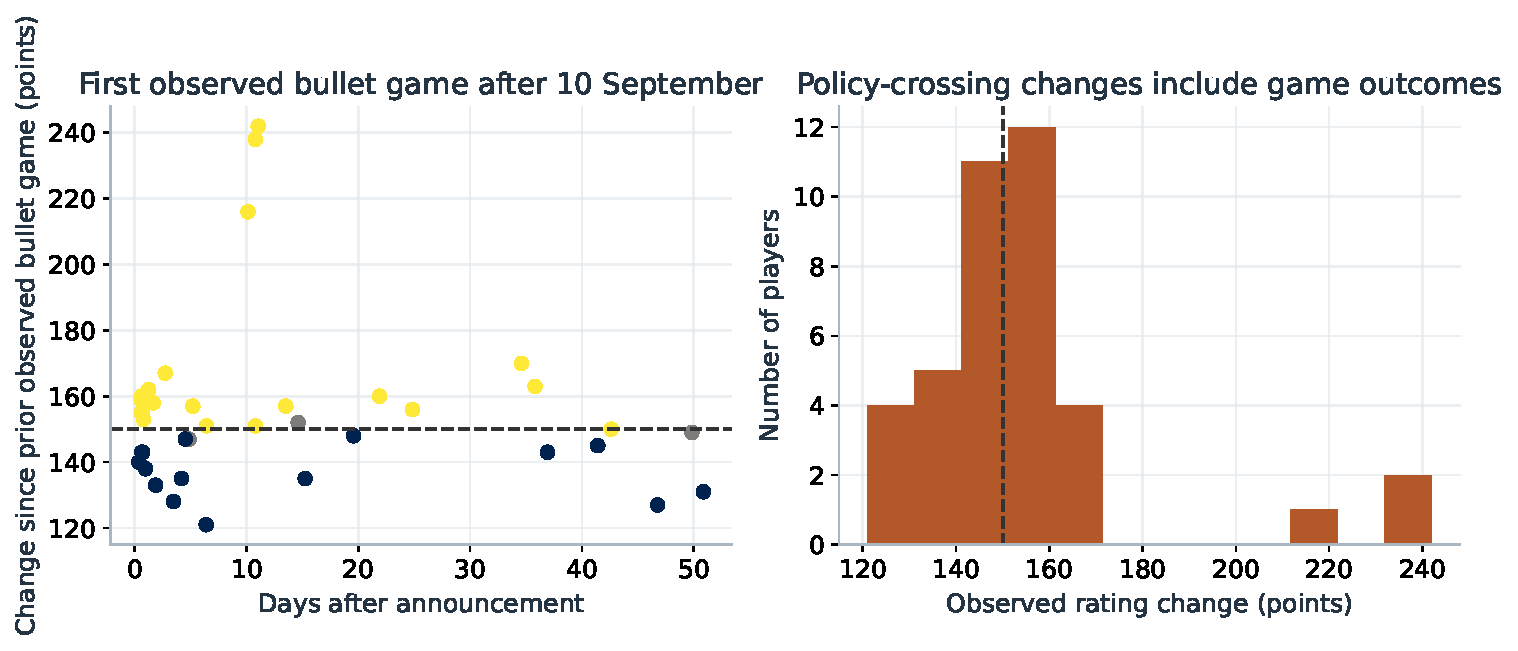
\includegraphics[width=\textwidth]{figures/08_rollout.pdf}\caption{First observed post-announcement bullet game minus the previous observed bullet rating. Scatter color encodes current score (0 = loss, 0.5 = draw, 1 = win); the offset line is 150. These changes include game updates and elapsed-time effects. Source: frozen cohort archives.}\end{figure}

The crossing statistic is not a clean measure of the administrative addition. It includes the result of the first post-event game, possibly multiple intervening rating adjustments, and delayed observation. A player can log in before playing, so first post-game observation is not the login time. The distribution is useful for consistency checks, and should not be converted into a staggered-adoption causal design without genuine treatment timestamps.

\section{Post-game information and outcome regressions}

\subsection{Retrospective association, not an operational forecast}

I fit a logistic regression to unique decisive games, with White win as the outcome, the post-game White-minus-Black rating gap in hundreds of points, pool indicators, post-period status, and a gap-by-post interaction. Draws are excluded, so the target is winning conditional on a decisive game, not expected score across all games. Standard errors are clustered by unordered opponent pair. Shared accounts across pairs and site-wide shocks remain sources of dependence.

The descriptive model is
\begin{equation}
\operatorname{logit}\Pr(W_g=1)=a+b\,\Delta R_g/100+\eta_c+d\,Post_g+q\,(\Delta R_g/100)Post_g.
\end{equation}
Because $\Delta R_g$ is measured after game $g$, $b$ and $q$ cannot be read as ex ante predictive accuracy or as causal effects of ratings on winning.

I fit the model using 55,783 decisive games from 21,949 observed opponent pairs. Its rating-gap coefficient is 0.724 log-odds per 100 post-game points, while the post-period interaction is 0.145 (p = 0.000). This is a parameter of a retrospective association.

\begin{table}[H]\centering\small\caption{Retrospective logistic regression; coefficients in log-odds, pair-clustered intervals}\begin{tabular}{p{5.5cm}rrr}\toprule

Term & Coefficient & SE & 95\% interval \\ \midrule

(Intercept) & 0.123 & 0.013 & 0.098 to 0.148 \\

gap100 & 0.724 & 0.020 & 0.686 to 0.763 \\

factor(time\_class)bullet & -0.018 & 0.021 & -0.059 to 0.023 \\

factor(time\_class)rapid & 0.045 & 0.112 & -0.174 to 0.264 \\

post & -0.026 & 0.020 & -0.066 to 0.013 \\

gap100:post & 0.145 & 0.033 & 0.080 to 0.210 \\

\bottomrule\end{tabular}\end{table}

\begin{figure}[H]\centering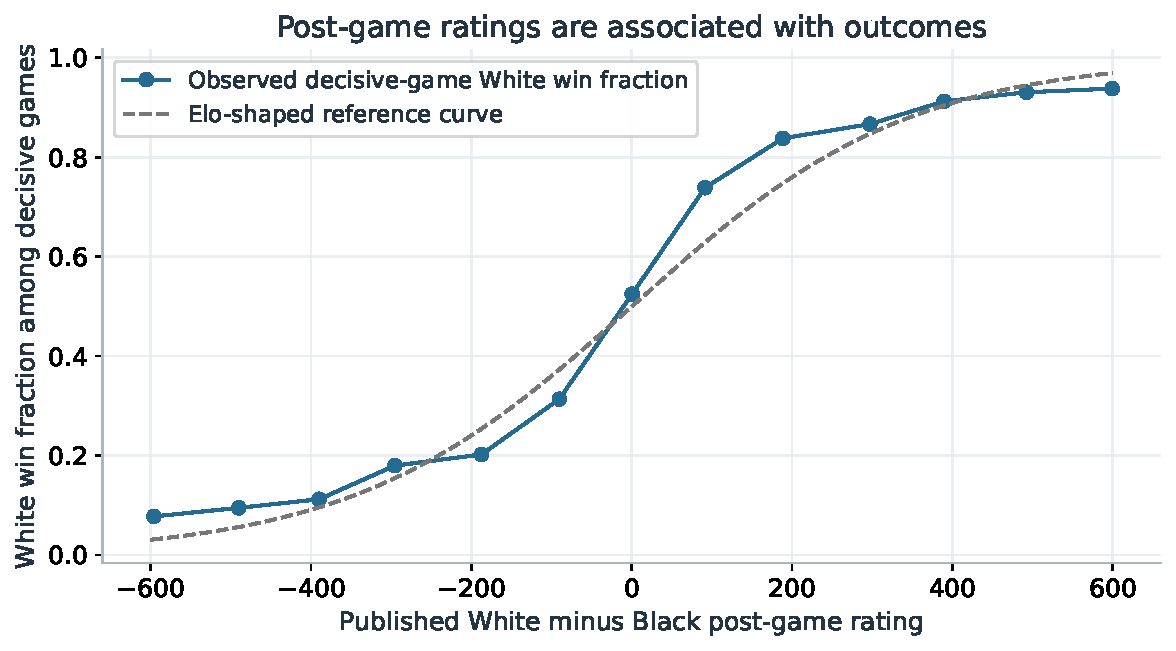
\includegraphics[width=\textwidth]{figures/09_retrospective_association.pdf}\caption{Binned White win fractions for decisive games against post-game rating differences, with at least 20 games per bin. The Elo-shaped line is an illustrative reference, not an ex ante calibration target for this conditional outcome. Source: unique cohort games.}\end{figure}

\subsection{An adjacent-rematch timing audit}

To quantify the timing problem without assuming symmetric rating exchanges, I locate a prior observed game between the same pair in the same speed class. I require the next game's start to be between 0 and 300 seconds after that game's end, and require that prior game to be the latest observed game for both accounts in that class. I then take both players' lagged ratings from the preceding game's post-game values, allowing color to switch.

At least one sampled account's complete monthly archive is available, but an unsampled opponent could have an unobserved intervening game elsewhere. Five-minute adjacency is therefore a defensible proxy for prior information, not a guarantee of exact pre-game state. Refunds and other updates may also occur. No opponent rating is reconstructed by forcing a zero-sum points exchange, since uncertainty-aware rating updates need not be symmetric.

\begin{table}[H]\centering\small\caption{Same decisive rematches, fixed Elo-shaped probability mapping; lower losses are better}\begin{tabular}{p{4.8cm}rrrr}\toprule

Rating source & Games & Accuracy & Brier & Log loss \\ \midrule

postgame & 21,674 & 68.0\% & 0.2134 & 0.6167 \\

lagged\_rematch & 21,674 & 60.0\% & 0.2336 & 0.6598 \\

\bottomrule\end{tabular}\end{table}

\begin{figure}[H]\centering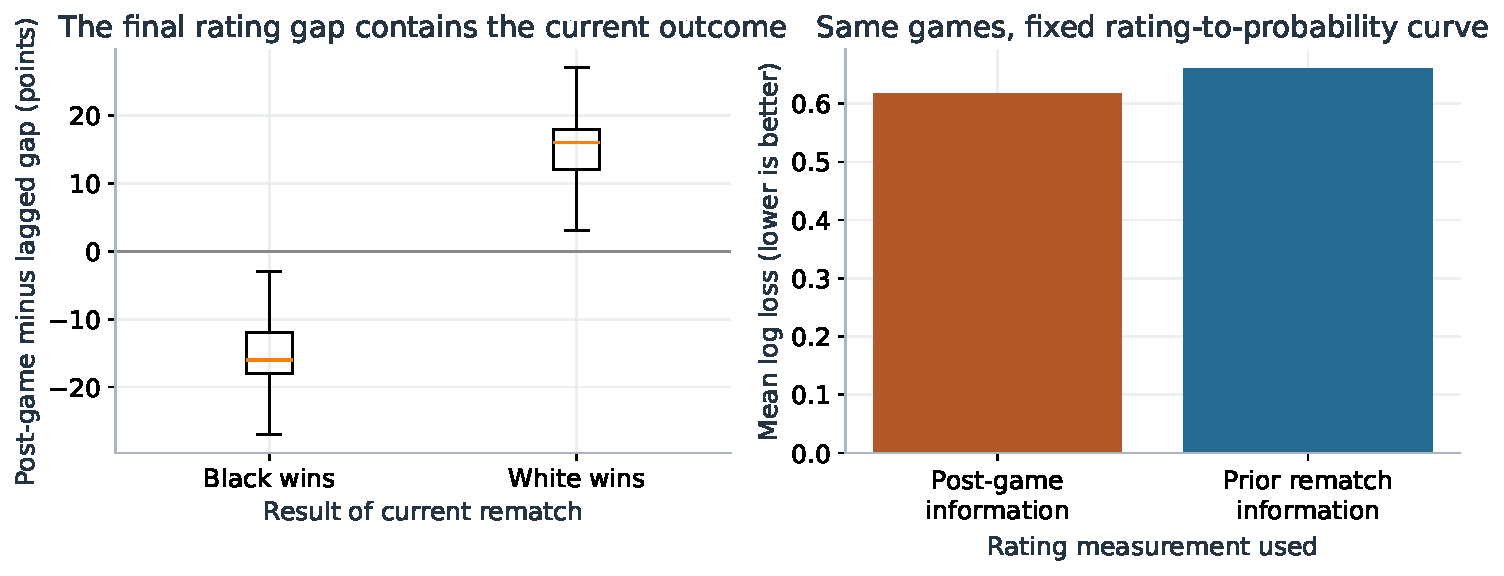
\includegraphics[width=\textwidth]{figures/10_leakage_audit.pdf}\caption{Left: post-game rating gap minus prior-rematch gap, grouped by the current result; boxplots omit outliers for display. Right: mean log loss using the same fixed probability curve on the same games. Source: adjacent decisive rematches, June--October 2020.}\end{figure}

Median gap updates are 16.0 points when White wins and -16.0 when Black wins. The equal-pair mean log-loss gain from post-game information is 0.0443, with percentile interval [0.0436, 0.0450], resampling 6,252 opponent-pair clusters 10,000 times. Game-weighted mean losses in the table and equal-pair differences target different weights.

This is a controlled timing comparison, not a learned prediction competition: the probability mapping is fixed and no model is tuned on future games. Its advantage is interpretability; its limitation is that an Elo-shaped curve is not a fitted Glicko forecast and the decisive-game restriction changes the target. The result shows how endpoint timing can alter apparent accuracy in this sample. It does not establish that every Chess.com prediction project is invalid, and it does not reproduce all conclusions of ChessIQ.

\section{Additional descriptive game analysis}

\begin{table}[H]\centering\small\caption{Unique-game descriptive statistics; length is the last full-move number in PGN}\begin{tabular}{lrrrr}\toprule

Pool & Unique games & Draw share & White mean score & Median length \\ \midrule

blitz & 40,684 & 10.3\% & 0.525 & 40.0 \\

bullet & 20,079 & 6.6\% & 0.519 & 41.0 \\

rapid & 716 & 24.6\% & 0.550 & 40.0 \\

\bottomrule\end{tabular}\end{table}

\begin{figure}[H]\centering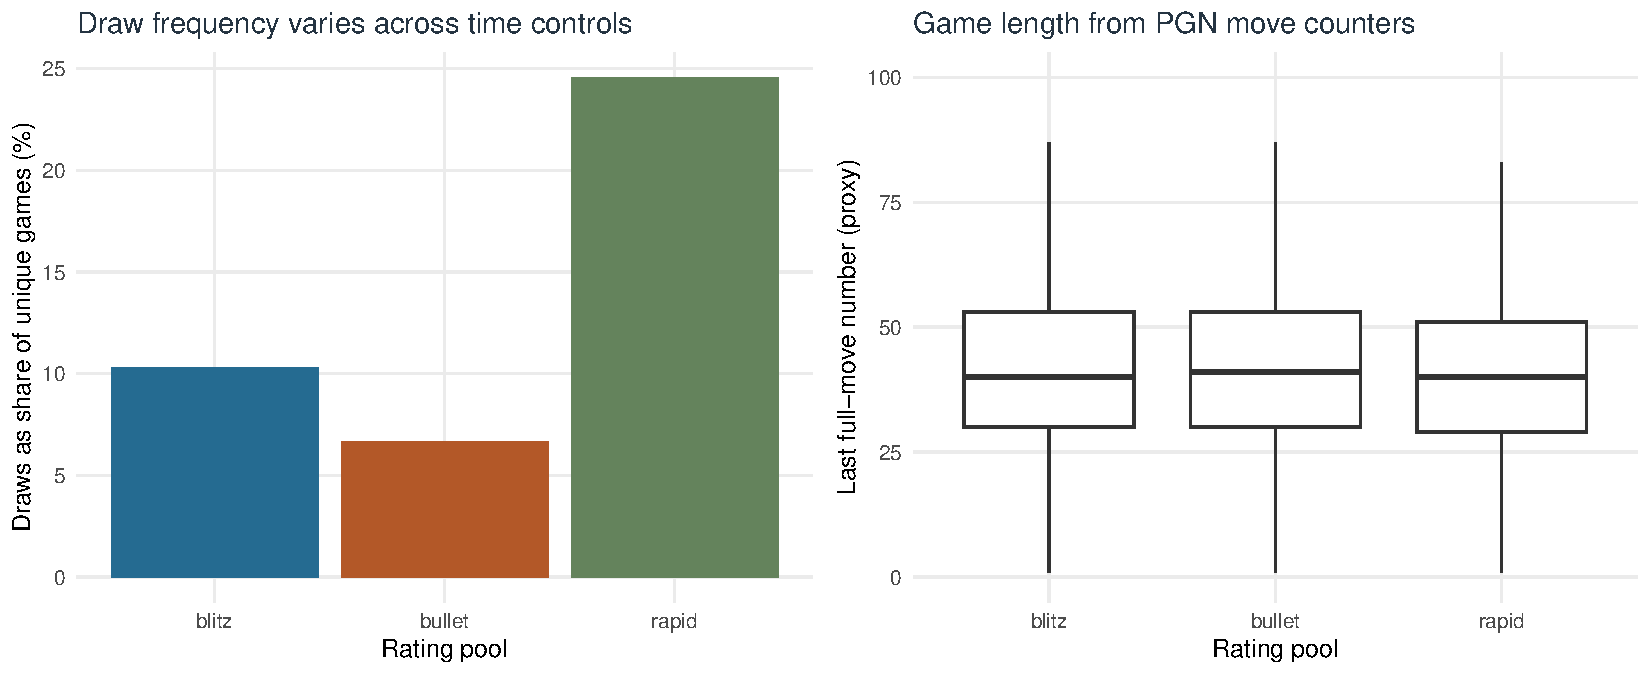
\includegraphics[width=\textwidth]{figures/11_game_characteristics.pdf}\caption{Draw shares and distributions of game length by speed class. Length is a PGN move-counter proxy rather than exact ply count; displayed boxplots omit outliers. Source: unique rated standard games, June--October 2020.}\end{figure}

Draw rates and game length supply useful context for the outcome analysis. They are not adjusted causal effects of longer thinking time: stronger players, different opponents, selected settings, and event formats may all vary across pools. Likewise, White's score in this cohort does not identify the causal advantage of color without evidence about color assignment and opponent selection.

\section{What can and cannot be concluded}

The strongest supported result is a reproducible measurement of rating behavior in a clearly defined historical cohort, together with explicit sensitivity to sample construction. The nominal 150-point policy is documented independently of the data, and an exactly common offset preserves relative rating gaps by algebra. These are compatible with a change in displayed rating scale without a demonstrated change in underlying ability.

A weaker, conditional statement is that the fitted bullet-versus-blitz panel contrast resembles an announcement effect under untreated parallel trends and negligible comparator spillovers. The simultaneous reform, uncertain treatment timing, incomplete activity support, current-title sampling, and shared pool shocks mean those assumptions remain contestable. I therefore interpret my DiD estimate conditionally and do not label it an identified average treatment effect.

Important limits are selection and survivorship; account-versus-person ambiguity; limited account clusters in tightly restricted settings; absent historical rating deviation and exact treatment receipt; rating refunds and possible retrospective archive changes; boundary-week exposure differences; outcome-dependent post-game measurement; rematch selection; and unobserved games by opponents outside sampled archives. Large game counts reduce some descriptive noise but do not remove these identification problems.

\subsection{A stronger future causal design}

A credible extension would first obtain exact account-level rebase timestamps and pre-update ratings, ideally from platform logs, plus a cohort frame fixed before the reform. It would record whether each opponent had already been rebased at match start. Relative-exposure contrasts could then examine temporary mismatches during rollout, with pre-specified short windows and explicit tests for selection into login timing.

Even that design would require handling interference: one player's rating is influenced by the opponents' states and by pool-wide matching. A randomized staged rollout, if a platform chose to conduct one, would offer stronger assignment evidence. A randomized experiment on rating display could study behavior while keeping the underlying matchmaking rating fixed; this is a proposal, not an experiment performed here.

\subsection{Other interesting questions supported by extensions of these data}

Three specific follow-ups are promising. First, estimate how incomplete opponent histories affect reconstructed pre-game ratings by varying observed rematch gaps and validating against a fully observed two-account subpanel. Second, decompose category migration using a pre-defined cohort of 10|0 specialists, rather than this GM-oriented sample. Third, study whether post-game information creates different apparent prediction gains for low- versus high-uncertainty accounts when historical RD becomes available. These questions add measurement and identification value instead of repeating a generic rating correlation.

\section{Reproducibility and delivery}

I provide a complete reproducible project containing frozen compressed API responses, processed datasets, request and hash logs, collection and analysis code, all generated figures in PDF and PNG, numerical result tables, this report's LaTeX source, the compiled PDF, dependency pins, verification utilities, and a README. Rebuilding analysis from the frozen data requires no Chess.com credentials and no fresh data download. Re-fetching is optional and can change the contemporary sampling frame.

From the repository root, restore the pinned R packages with \texttt{Rscript scripts/setup.R}, run \texttt{Rscript scripts/analyze.R}, then run \texttt{Rscript scripts/verify.R} and \texttt{Rscript scripts/build\_report.R}. Compile from the report folder using \texttt{tectonic report.tex}; an ordinary XeLaTeX installation can also compile the source twice. The delivered report is actually typeset from LaTeX, with vector figure inputs. The self-contained compiler used for delivery was Tectonic 0.17.0; portable Palatino, Helvetica, and Courier TeX fonts avoid dependence on installed desktop fonts.

I release my original code and report text under an MIT license. Public platform data are attributed separately and are not relicensed by the code license. The source archives include public game handles and URLs for provenance; no private chats, emails, or authentication tokens were collected. The repository contains the source files, frozen data, estimates, figures and compiled report needed to inspect and reproduce my analysis.

\clearpage\appendix

\section{Variable definitions and analytical checks}

\begin{table}[H]\centering\small\caption{Core data dictionary; full columns are retained in processed CSV files}\begin{tabular}{p{4.4cm}p{9cm}}\toprule

Variable & Definition / timing \\ \midrule

\texttt{game\_id} & UUID, with public game URL as fallback \\

\texttt{rating} & Focal account rating after the game, from JSON \\

\texttt{white\_score} & White result: 1, 0.5, 0; unique-game unit \\

\texttt{score} & Focal account score, adjusted for color \\

\texttt{event\_week} & Floor of elapsed UTC time / seven days from 10 Sep \\

\texttt{post} & Descriptive indicator for completion on/after 10 Sep \\

\texttt{treat} & Bullet indicator times post, with week 0 omitted \\

\texttt{unit} & Account-by-rating-pool panel identifier \\

\texttt{rating\_change} & Current minus prior observed focal rating in same pool \\

\texttt{lag\_gap} & White minus Black ratings from previous observed rematch \\

\texttt{pair} & Unordered normalized account pair \\

\texttt{moves\_proxy} & Last numeric full-move counter in PGN \\

\bottomrule\end{tabular}\end{table}

Verification checks include uniqueness of game identifiers; one or two focal rows per unique sampled game; valid score and class values; temporal ordering for prior-rematch information; non-overlapping prior/current game times for the rematch audit; sufficient policy variation in the panel; full numerical output without invented rows; raw-response hash consistency; expected figure existence; and PDF text and page rendering checks. The verification file reports actual checks rather than substituting test outcomes for identification arguments.

\section{Source notes and references}

I consulted the web sources on 11 October 2026. Policy and endpoint semantics rely on the platform's own documentation. Prior applied work is identified by direct author pages or repositories. Literature-search limitations are stated in Section 2. The frozen data and request log are the source for all empirical counts and estimates; figures 12 and 13 are explanatory diagrams.

\begin{thebibliography}{99}
\bibitem{policy} Chess.com (2020). \emph{[Updated] 10 Minute Chess Now Rapid Rated, Bullet Ratings Increased}, 10 September. \url{https://www.chess.com/news/view/10-minute-chess-now-rapid-rated-bullet-ratings-increased}.
\bibitem{pubapi} Chess.com. \emph{Published-Data API}, including monthly archives, game result codes, rating timing, and serial access. \url{https://www.chess.com/news/view/published-data-api}.
\bibitem{chessratings} Chess.com Help Center. \emph{How do ratings work on Chess.com?} \url{https://support.chess.com/en/articles/8566476-how-do-ratings-work-on-chess-com}.
\bibitem{lichessratings} Lichess. \emph{Chess rating systems}. \url{https://lichess.org/page/rating-systems}.
\bibitem{glicko} Glickman, M. E. \emph{The Glicko system}. Technical specification. \url{https://www.glicko.net/glicko/glicko.pdf}.
\bibitem{sharma} Sharma, T. (2023). \emph{Predicting Rapid Ratings on Chess.com: A Data-Driven Approach}. Author's Chess.com blog, 22 May. \url{https://www.chess.com/blog/tusharsharma96/predicting-rapid-ratings-on-chess-com-a-data-driven-approach}.
\bibitem{chessiq} keyurc2332. \emph{ChessIQ: Chess outcome prediction, and the three data leaks that made it look possible}. Public repository; consulted version at retrieval, not a peer-reviewed article. \url{https://github.com/keyurc2332/ChessIQ}.
\bibitem{smerdon} Smerdon, D. (2021). \emph{The Fighting Chess Index}, 10 June. Author's methodological article. \url{https://www.davidsmerdon.com/?p=2168}.
\bibitem{bertrand} Bertrand, M., Duflo, E., and Mullainathan, S. (2004). How Much Should We Trust Differences-in-Differences Estimates? \emph{Quarterly Journal of Economics}, 119(1), 249--275. Working-paper record: \url{https://www.nber.org/papers/w8841}.
\bibitem{conley} Conley, T. and Taber, C. (2005). \emph{Inference with Difference in Differences with a Small Number of Policy Changes}. NBER Technical Working Paper 312. \url{https://www.nber.org/papers/t0312}.
\bibitem{roth} Roth, J. (2022). Pretest with Caution: Event-Study Estimates after Testing for Parallel Trends. \emph{American Economic Review: Insights}, 4(3), 305--322. Author manuscript: \url{https://www.jonathandroth.com/assets/files/roth_pretrends_testing.pdf}.
\bibitem{rstats} R Core Team. \emph{R: A Language and Environment for Statistical Computing}. \url{https://www.r-project.org/}.
\bibitem{zeileis} Zeileis, A. \emph{Econometric Computing with HC and HAC Covariance Matrix Estimators}. Technical vignette. \url{https://cran.r-project.org/web/packages/sandwich/vignettes/sandwich.pdf}.
\end{thebibliography}
\end{document}

